\chapter{控制系统的状态空间模型}
\label{chap:state-space-model}

\section{状态变量与状态空间模型}

\dfn{状态（State）}{给定时刻的状态 $x(t_0)$ 和此后的输入 $u(t)$，即可确定系统此后的状态和输出。用来描述内部动态的独立变量组成状态向量，这些变量张成的空间称为状态空间。}

连续时间线性定常系统写为
\[
\dot x=Ax+Bu,\qquad y=Cx+Du.
\]
若 $x\in\mathbb R^n$、$u\in\mathbb R^r$、$y\in\mathbb R^m$，则 $A,B,C,D$ 分别为 $n\times n$、$n\times r$、$m\times n$ 和 $m\times r$ 矩阵。$D$ 表示输入到输出的直接传递。单输入单输出情形有 $r=m=1$，因此 $B$ 是列向量，$C$ 是行向量，$D$ 是标量。时变系统的矩阵允许显含 $t$。一般非线性系统写为 $\dot x=f(x,u,t)$、$y=g(x,u,t)$。

\nt{\textbf{讲义思考（第5页）} 平面匀速运动取 $x=(p_x,p_y,v_x,v_y)^{\mathsf T}$，有 $\dot p_x=v_x$、$\dot p_y=v_y$、$\dot v_x=\dot v_y=0$。当速度由题意预先给定，且所有可能轨迹共享该速度时，只需记录两个位置分量。}
\nt{\textbf{讲义思考（第15页）}\quad 单输入单输出线性定常系统可写成 $\dot x_i=\sum_{j=1}^n a_{ij}x_j+b_i u$（$i=1,\ldots,n$），$y=\sum_{j=1}^n c_jx_j+du$。比较输入、输出通道数即可确定 $B,C,D$ 的形状。}

\section{模拟结构图与机理建模}

电路常选独立的电容电压和电感电流，写出 $i_C=C\dot u_C$、$u_L=L\dot i_L$，再用基尔霍夫电流及电压定律消去其余变量。机械系统常把广义位移和广义速度配对，利用力或力矩平衡解出加速度。平衡点 $(x_e,u_e)$ 满足 $f(x_e,u_e)=0$，在其附近以偏差量为变量时，一阶近似的 $A,B,C,D$ 分别是 $f,g$ 对 $x,u$ 的雅可比矩阵在平衡点处的取值。

读模拟结构图时，先为各积分器的输出编号，再沿每个积分器的输入端往回读各条支路的增益与符号。第 $i$ 个积分器的输入是 $\dot x_i$，相应系数组成 $A,B$ 的第 $i$ 行。最后沿输出端读取 $C,D$。


\dfn{线性化}{对于 $\dot x=f(x,u),\ y=g(x,u)$，取 $f(x_e,u_e)=0$，$y_e=g(x_e,u_e)$。令 $\Delta x=x-x_e$、$\Delta u=u-u_e$。忽略二阶及更高阶小量后有
\[
\Delta\dot x=f_x|_e\,\Delta x+f_u|_e\,\Delta u,\qquad
\Delta y=g_x|_e\,\Delta x+g_u|_e\,\Delta u.
\]
建立模型后，仍应检查线性化点是否符合题设和所选工作范围。}

\begin{center}
\begin{tikzpicture}[>=Stealth,block/.style={draw,rounded corners=1pt,minimum width=9mm,minimum height=7mm},
    sum/.style={draw,circle,inner sep=0pt,minimum size=5mm}]
    \node[block] (b) at (1.25,0) {$B(t)$};
    \node[sum] (sx) at (2.65,0) {$+$};
    \node[block] (i) at (4.55,0) {$\int$};
    \node[block] (c) at (6.55,0) {$C(t)$};
    \node[sum] (sy) at (8,0) {$+$};
    \node[block] (a) at (4,-1.05) {$A(t)$};
    \node[block] (d) at (4.6,1.05) {$D(t)$};
    \draw[->] (0,0) node[left] {$u$} -- (b);
    \draw[->] (b) -- (sx);
    \draw[->] (sx) -- node[above] {$\dot x$} (i);
    \draw[->] (i) -- node[above] {$x$} (c);
    \draw[->] (c) -- (sy);
    \draw[->] (sy) -- (8.8,0) node[right] {$y$};
    \draw[->] (5.55,0) |- (a);
    \draw[->] (a) -| (sx);
    \draw[->] (.44,0) |- (d);
    \draw[->] (d) -| (sy);
    \fill (.44,0) circle[radius=1pt];
    \fill (5.55,0) circle[radius=1pt];
\end{tikzpicture}

\small 线性系统的模拟结构（据讲义第22页图2-5重绘）
\end{center}

\subsection{读写模拟结构图}

\ex{讲义例2-1（第25--26页）\quad 由模型画模拟结构图}{
已知
\[
\dot x=\begin{bmatrix}0&a&0\\0&b&c\\d&0&e\end{bmatrix}x+
\begin{bmatrix}0\\0\\f\end{bmatrix}u,\qquad
y=\begin{bmatrix}1&0&0\end{bmatrix}x.
\]
画出模拟结构图，并从图反读其状态方程。}

\nt{\textbf{知识点}\quad 积分器的输入与输出、系数符号与信号流向。}

\sol 从最后一个状态开始，$fu$、$dx_1$ 与 $ex_3$ 先相加，经积分器得到 $x_3$。$cx_3+bx_2$ 积分得到 $x_2$，$ax_2$ 积分得到 $x_1$，直接取 $y=x_1$。
\begin{center}
\begin{tikzpicture}[>=Stealth,block/.style={draw,minimum width=7mm,minimum height=6mm},
    sum/.style={draw,circle,inner sep=0pt,minimum size=5mm}]
    \node[block] (f) at (.75,0) {$f$};
    \node[sum] (s3) at (1.55,0) {$+$};
    \node[block] (i3) at (2.6,0) {$\int$};
    \node[block] (c) at (3.85,0) {$c$};
    \node[sum] (s2) at (4.65,0) {$+$};
    \node[block] (i2) at (5.7,0) {$\int$};
    \node[block] (a) at (6.95,0) {$a$};
    \node[block] (i1) at (8,0) {$\int$};
    \node[block] (e) at (2.4,-.9) {$e$};
    \node[block] (b) at (5.5,-.9) {$b$};
    \node[block] (d) at (5,1.05) {$d$};
    \draw[->] (0,0) node[left] {$u$} -- (f);
    \draw[->] (f) -- (s3);
    \draw[->] (s3) -- node[above] {$\dot x_3$} (i3);
    \draw[->] (i3) -- node[above] {$x_3$} (c);
    \draw[->] (c) -- (s2);
    \draw[->] (s2) -- node[above] {$\dot x_2$} (i2);
    \draw[->] (i2) -- node[above] {$x_2$} (a);
    \draw[->] (a) -- node[above] {$\dot x_1$} (i1);
    \draw[->] (i1) -- node[above] {$x_1$} (9.25,0) node[right] {$y$};
    \draw[->] (3.2,0) |- (e);
    \draw[->] (e) -| (s3);
    \draw[->] (6.3,0) |- (b);
    \draw[->] (b) -| (s2);
    \draw[->] (8.72,0) |- (d);
    \draw[->] (d) -| (s3);
    \foreach \x in {3.2,6.3,8.72} \fill (\x,0) circle[radius=1pt];
\end{tikzpicture}
\end{center}
沿三个积分器的输入端反查，分别得到 $\dot x_1=ax_2$、$\dot x_2=bx_2+cx_3$ 和 $\dot x_3=dx_1+ex_3+fu$。

\ex{讲义第26页指定练习\quad 教材第17页图1.7(b)\quad 从模拟结构图列方程}{
教材图1.7(b) 将前向通道 $K_1/(T_1s+1)$、$K_2/(T_2s+1)$ 和 $K_3/(T_3s)$ 依次串联，输出 $y$ 经增益 $K_4$ 反馈至输入的负端。按图自左向右取三个积分器的输出为 $x_3,x_2,x_1$，求状态空间模型。
\begin{center}
\begin{tikzpicture}[>=Stealth,x=.91cm,
    block/.style={draw,minimum width=8mm,minimum height=7mm},
    integ/.style={draw,minimum width=5mm,minimum height=7mm},
    sum/.style={draw,circle,inner sep=0pt,minimum size=5mm}]
    \node[sum] (s0) at (.4,0) {$\sum$};
    \node[block] (b1) at (1.42,0) {$\tfrac{K_1}{T_1}$};
    \node[sum] (s3) at (2.46,0) {$\sum$};
    \node[integ] (i3) at (3.45,0) {$\int$};
    \node[block] (b2) at (4.66,0) {$\tfrac{K_2}{T_2}$};
    \node[sum] (s2) at (5.7,0) {$\sum$};
    \node[integ] (i2) at (6.69,0) {$\int$};
    \node[block] (b3) at (7.9,0) {$\tfrac{K_3}{T_3}$};
    \node[integ] (i1) at (8.95,0) {$\int$};
    \node[block] (r3) at (3.24,-1.28) {$\tfrac1{T_1}$};
    \node[block] (r2) at (6.48,-1.28) {$\tfrac1{T_2}$};
    \node[block] (r0) at (5,-2.42) {$K_4$};
    \draw[->] (-.56,0) node[left] {$u$} -- node[above,pos=.75] {$+$} (s0);
    \draw[->] (s0) -- (b1);
    \draw[->] (b1) -- node[above] {$+$} (s3);
    \draw[->] (s3) -- node[above] {$\dot x_3$} (i3);
    \draw[->] (i3) -- node[above] {$x_3$} (b2);
    \draw[->] (b2) -- node[above] {$+$} (s2);
    \draw[->] (s2) -- node[above] {$\dot x_2$} (i2);
    \draw[->] (i2) -- node[above] {$x_2$} (b3);
    \draw[->] (b3) -- node[above] {$\dot x_1$} (i1);
    \draw[->] (i1) -- node[above] {$x_1$} (10.35,0) node[right] {$y$};
    \draw[->] (3.99,0) |- (r3);
    \draw[->] (r3) -| node[near end,left] {$-$} (s3);
    \draw[->] (7.23,0) |- (r2);
    \draw[->] (r2) -| node[near end,left] {$-$} (s2);
    \draw[->] (9.68,0) |- (r0);
    \draw[->] (r0) -| node[near end,left] {$-$} (s0);
    \foreach \x in {3.99,7.23,9.68} \fill (\x,0) circle[radius=1pt];
\end{tikzpicture}
\end{center}
}

\nt{\textbf{知识点} 将一阶环节改写为积分器结构，沿负反馈支路读取系数，保持题设状态编号。}

\sol 输入到第一个环节的误差信号为 $e=u-K_4x_1$。前两个一阶惯性环节分别满足 $T_1\dot x_3+x_3=K_1 e$ 和 $T_2\dot x_2+x_2=K_2x_3$。最后的积分环节满足 $T_3\dot x_1=K_3x_2$。由于输出就是 $x_1$，所以
\[
\dot x=\begin{bmatrix}
0&K_3/T_3&0\\
0&-1/T_2&K_2/T_2\\
-K_1K_4/T_1&0&-1/T_1
\end{bmatrix}x+
\begin{bmatrix}0\\0\\K_1/T_1\end{bmatrix}u,\qquad
y=\begin{bmatrix}1&0&0\end{bmatrix}x.
\]
讲义第26页用符号增益 $a,b,c,d,e,f$ 表示图中各支路，对应 $\dot x_1=ax_2$、$\dot x_2=bx_2+cx_3$、$\dot x_3=dx_1+ex_3+fu$。反馈方向已经包含在 $b,d,e$ 的取值中。

\Needspace{22\baselineskip}
\subsection{纸质练习}

\ex{纸质练习一\quad 由反馈结构图建立状态空间模型}{
按图中的 $x_1,x_2$ 选取状态，求输入 $u$ 到输出 $y$ 的状态空间表达式。
\begin{center}
\begin{tikzpicture}[>=Stealth,
    block/.style={draw, minimum width=1.65cm, minimum height=0.95cm},
    sum/.style={draw,circle,inner sep=0pt,minimum size=6mm}]
    \node[sum] (sum) at (0,0) {$\scriptstyle\sum$};
    \node[block] (plant) at (2.35,0) {$\dfrac{k}{s+2}$};
    \node[block] (sensor) at (2.35,-1.4) {$\dfrac{1}{s+1}$};
    \draw[->] (-1.4,0) node[above] {$u$} -- node[above,pos=.82] {$+$} (sum);
    \draw[->] (sum) -- (plant);
    \draw[->] (plant) -- (4.9,0) node[right] {$y$};
    \fill (3.9,0) circle[radius=1.2pt] node[above] {$x_1$};
    \draw[->] (3.9,0) |- (sensor.east);
    \draw[->] (sensor.west) -| node[pos=.3,above] {$x_2$}
        node[pos=.86,right] {$-$} (sum.south);
\end{tikzpicture}
\end{center}
}

\nt{\textbf{知识点}\quad 一阶环节的微分方程、负反馈求和、状态方程与输出方程。}

\sol 先读求和点。前向环节的输入为 $u-x_2$，其输出为 $x_1$。反馈环节的输入为 $x_1$，输出为 $x_2$，因此在时域中有
\[
    \dot x_1+2x_1=k(u-x_2),\qquad \dot x_2+x_2=x_1.
\]
输出从前向环节末端引出，故 $y=x_1$。整理得
\[
    \boxed{
    \dot x=\begin{bmatrix}-2&-k\\1&-1\end{bmatrix}x
           +\begin{bmatrix}k\\0\end{bmatrix}u,\qquad
    y=\begin{bmatrix}1&0\end{bmatrix}x,\quad D=0.}
\]
检验时可在零初始条件下消去 $X_2=X_1/(s+1)$，得到
\[
    \frac{Y(s)}{U(s)}=\frac{k(s+1)}{(s+2)(s+1)+k}.
\]
这与把两个一阶环节直接按负反馈连接所得的闭环传递函数一致。


\subsection{由物理元件和受力关系建模}

\ex{讲义电路例题（第11--13页）\quad 串联 RLC 电路}{
电阻 $R$、电感 $L$ 和电容 $C$ 串联，由电压源 $u_i$ 驱动。电流 $i_L$ 从电源正端经 $R,L$ 流入电容正端。以 $u_i$ 为输入、电容电压 $u_C$ 为输出，建立状态空间模型，并在零初值下求传递函数及阶数。
\begin{center}
\begin{tikzpicture}[>=Stealth]
    \draw (0,0) -- (0,.55) (0,1.45) -- (0,2) -- (1.1,2)
        (2,2) -- (2.8,2) (3.8,2) -- (4.7,2) -- (4.7,1.2)
        (4.7,.95) -- (4.7,0) -- (0,0);
    \draw (0,1) circle[radius=.45];
    \node[left] at (-.45,1) {$u_i$};
    \node at (0,1.19) {$+$};
    \node at (0,.81) {$-$};
    \draw (1.1,1.87) rectangle (2,2.13);
    \node[above] at (1.55,2.15) {$R$};
    \foreach \a in {2.8,3.05,3.3,3.55} \draw (\a,2) arc[start angle=180,end angle=0,radius=.125];
    \node[above] at (3.3,2.16) {$L$};
    \draw (4.46,1.2)--(4.94,1.2) (4.46,.95)--(4.94,.95);
    \node[right] at (4.98,1.08) {$C,\ u_C$};
    \node at (5.02,1.45) {$+$};
    \node at (5.02,.71) {$-$};
    \draw[->] (.6,1.61) -- (1.35,1.61) node[right] {$i_L$};
\end{tikzpicture}
\end{center}
}

\nt{\textbf{知识点}\quad 用电容电压与电感电流记录储能状态，按零初值求传递函数。}

\sol 选取 $x_1=u_C$、$x_2=i_L$。从 $C\dot u_C=i_L$ 和 $L\dot i_L=u_i-Ri_L-u_C$ 可得
\[
\dot x=\begin{bmatrix}0&1/C\\-1/L&-R/L\end{bmatrix}x+
\begin{bmatrix}0\\1/L\end{bmatrix}u_i,\qquad y=\begin{bmatrix}1&0\end{bmatrix}x.
\]
再消去 $i_L$，得 $LC\ddot u_C+RC\dot u_C+u_C=u_i$。零初始条件下 $U_C(s)/U_i(s)=1/(LCs^2+RCs+1)$。当 $L,C>0$ 时分母二次且无对消，传递函数为二阶。

\ex{讲义例题\quad 弹簧、质量体与阻尼器（第30--33页）}{
质量为 $m$ 的小车沿水平轨道运动，两侧分别通过刚度为 $k$ 的弹簧和黏性阻尼系数为 $f$ 的阻尼器与固定支座相连。外力 $u(t)$ 与位移 $y(t)$ 的正方向均向右。力施加前小车在静止平衡位置，$y$ 从该位置计量。建立以 $u$ 为输入、$y$ 为输出的状态空间模型。
\begin{center}
\begin{tikzpicture}[>=Stealth]
    \draw[gray] (-3.15,.92) |- (3.15,-.45) -- (3.15,.92);
    \foreach \x in {-3.15,3.15} {
        \foreach \h in {0,.21,.42,.63,.84} {\draw[gray] (\x,\h) -- ++(-.15,-.15);}
    }
    \draw[thick,fill=mytheorembg] (-.68,-.14) rectangle (.68,.75);
    \node at (0,.31) {$m$};
    \draw[thick] (-.35,-.29) circle[radius=.15] (.35,-.29) circle[radius=.15];
    \draw[myb,thick] (-3.15,.31) -- (-2.7,.31) --
       (-2.54,.49) -- (-2.32,.13) -- (-2.1,.49) -- (-1.88,.13) --
       (-1.66,.49) -- (-1.44,.13) -- (-1.28,.31) -- (-.68,.31);
    \node[below,myb] at (-2.09,.13) {$k$};
    \draw[myb,thick] (.68,.31) -- (1.73,.31) (1.73,.09) -- (1.73,.53)
       (1.55,.01) -- (2.17,.01) -- (2.17,.61) -- (1.55,.61)
       (2.17,.31) -- (3.15,.31);
    \node[below,myb] at (1.92,0) {$f$};
    \draw[->,thick,myr] (-1.5,.98) -- node[above] {$u(t)$} (-.65,.98);
    \draw[->] (.68,1.16) -- node[above] {$y(t)$} (1.8,1.16);
\end{tikzpicture}
\end{center}
}

\nt{\textbf{知识点}\quad 牛顿第二定律、黏性阻尼、用位移与速度建立二阶系统。}

\sol 沿 $y$ 的正方向列力平衡。外力为 $u$，弹簧的回复力是 $-ky$，阻尼力是 $-f\dot y$，所以
\[
    m\ddot y=u-f\dot y-ky .
\]
取 $x_1=y$、$x_2=\dot y$，得到 $\dot x_1=x_2$、$\dot x_2=-(k/m)x_1-(f/m)x_2+u/m$。于是
\[
    \dot x=\begin{bmatrix}0&1\\-k/m&-f/m\end{bmatrix}x
    +\begin{bmatrix}0\\1/m\end{bmatrix}u,\qquad
    y=\begin{bmatrix}1&0\end{bmatrix}x,\qquad D=0 .
\]
题设的静止平衡初态对应 $x(0)=0$。消去 $x_2$ 可回到原动力学式。若改为测加速度，输出是
$\ddot y=-(k/m)x_1-(f/m)x_2+u/m$，此时 $A,B$ 相同，输出矩阵改为 $C=[-k/m\ \ {-f/m}]$，且 $D=1/m$。

\begin{note}
同一物理系统可测位移、速度或加速度。先由机理定出 $A,B$，然后按题目的测量量写 $C,D$。常见平衡规律有电路的电压/电流定律、机械系统的力/力矩平衡，以及流体和热过程中的物料/能量守恒。
\end{note}


\ex{习题1（习题课第1页）\quad RLC 电路建模}{
如图，RLC 电路中含电压源 $u_1(t)$ 和电流源 $u_2(t)$。试建立以两源为输入、电感 $L$ 上的电压 $u_L(t)$ 为输出的状态空间模型。
\par\smallskip
\begin{center}
    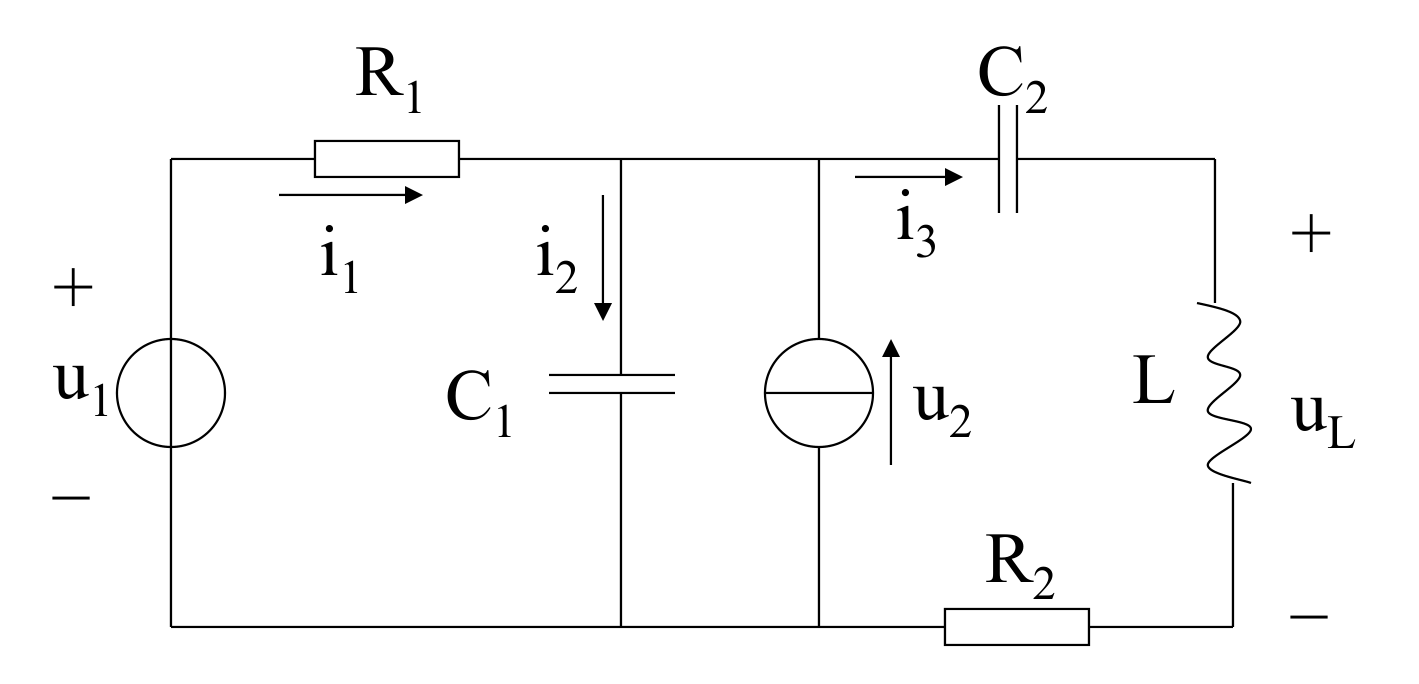
\includegraphics[width=0.79\linewidth]{ch02-rlc-circuit.png}
\end{center}
}

\nt{\textbf{知识点} 独立储能元件的状态选取、节点电流定律、回路电压定律、电感电压的被动符号约定。}

\sol 令 $x_1=u_{C_1}$（上正下负）、$x_2=u_{C_2}$（左正右负）、$x_3=i_3$，$u=[u_1,u_2]^{\mathsf T}$。电流源箭头朝上，所以在电路上方的公共节点有 $i_1+u_2=i_2+i_3$。左支路给出 $i_1=(u_1-x_1)/R_1$，而 $i_2=C_1\dot x_1$，因此
\[
C_1\dot x_1=\frac{u_1-x_1}{R_1}+u_2-x_3.
\]
从右支路可读出 $C_2\dot x_2=x_3$。沿 $C_2$、$L$、$R_2$ 所在回路列电压方程，得
\[
x_1=x_2+u_L+R_2x_3,\qquad u_L=L\dot x_3.
\]
整理得
\[
\dot x=
\begin{bmatrix}
-\frac1{R_1C_1}&0&-\frac1{C_1}\\
0&0&\frac1{C_2}\\
\frac1L&-\frac1L&-\frac{R_2}L
\end{bmatrix}x+
\begin{bmatrix}
\frac1{R_1C_1}&\frac1{C_1}\\
0&0\\
0&0
\end{bmatrix}u,\qquad
y=\begin{bmatrix}1&-1&-R_2\end{bmatrix}x.
\]
输出由三个状态量直接求得，故 $D=[0\quad 0]$。

\section{由输入输出关系建立状态空间模型}

给定 $a(s)=s^n+a_{n-1}s^{n-1}+\cdots+a_0$。引入中间量 $v$，使 $a(\mathrm d/\mathrm dt)v=u$，再取 $x=(v,\dot v,\ldots,v^{(n-1)})^{\mathsf T}$。状态矩阵的超对角线为 1，末行为 $[-a_0,\ldots,-a_{n-1}]$，而 $B=e_n$。设传递函数 $G(s)=N(s)/a(s)$，先写 $G(s)=d+\widetilde N(s)/a(s)$，其中 $\deg\widetilde N<n$。将 $\widetilde N(s)=\sum_{i=0}^{n-1}b_is^i$ 的系数按次数从低到高排成 $C=[b_0,\ldots,b_{n-1}]$，得 $y=Cx+du$。

\nt{若原微分方程的右端只有 $bu$，可直接取 $x_1=y$、$x_2=\dot y$ 等，此时 $B=be_n$。右端含输入导数时，可按上述传递函数法实现，也可重定义各阶状态以吸收输入导数，见习题3。}

从部分分式出发，单极点项 $c/(s-\lambda)$ 对应 $\dot x=\lambda x+u$、$y=cx$。对 $q$ 重极点，设 $J_q=\lambda I+N$，$N$ 的超对角线为 1。取该支路的 $B=e_q$，有
\[
(sI-J_q)^{-1}e_q=
\begin{bmatrix}
(s-\lambda)^{-q}\\ (s-\lambda)^{-(q-1)}\\ \vdots\\ (s-\lambda)^{-1}
\end{bmatrix}.
\]
因此 $C$ 按分母幂次从高到低取相应的部分分式系数。各支路的输出相加，另加直联项 $Du$。
\nt{\textbf{建模顺序}\quad 先把分母最高次项系数化为 1。只求零初值输入输出关系时，可借助传递函数重选状态；题给非零初值时，必须根据所选状态与 $y,u$ 的关系换算初值。若输入导数的最高次数与输出阶数相同，需要先抽出直联项 $D$。}

\subsection{微分方程的直接实现}

\ex{讲义例2-2和例2-4（第46--47、68--70页）\quad 同一系统的两种实现}{
将 $y^{(3)}+6\ddot y+11\dot y+6y=2u$ 变换为状态空间模型。再用部分分式法，将其零初值传递函数 $G(s)=2/(s^3+6s^2+11s+6)$ 变换为状态空间模型。}

\nt{\textbf{知识点}\quad 相变量实现、单极点留数、状态坐标的非唯一性。}

\sol \textbf{例2-2。} 取 $x=(y,\dot y,\ddot y)^{\mathsf T}$，先写 $\dot x_1=x_2,\dot x_2=x_3$，由原方程得 $\dot x_3=2u-6x_1-11x_2-6x_3$。即
\[
A=\begin{bmatrix}0&1&0\\0&0&1\\-6&-11&-6\end{bmatrix},\quad
B=\begin{bmatrix}0\\0\\2\end{bmatrix},\quad C=[1\;0\;0],\quad D=0.
\]
从 $2u-6x_1-11x_2-6x_3$ 起串接三个积分器，其输出依次为 $x_3,x_2,x_1=y$，各状态乘相应负系数回到首个求和点。
\begin{center}
\begin{tikzpicture}[>=Stealth,block/.style={draw,minimum width=7mm,minimum height=6mm},
    sum/.style={draw,circle,inner sep=0pt,minimum size=5mm}]
    \node[block] (b) at (.85,0) {$2$};
    \node[sum] (s) at (1.95,0) {$+$};
    \node[block] (i3) at (3.4,0) {$\int$};
    \node[block] (i2) at (4.9,0) {$\int$};
    \node[block] (i1) at (6.4,0) {$\int$};
    \node[block] (r3) at (3.07,-.7) {$-6$};
    \node[block] (r2) at (3.07,-1.47) {$-11$};
    \node[block] (r1) at (3.07,-2.24) {$-6$};
    \draw[->] (0,0) node[left] {$u$} -- (b);
    \draw[->] (b) -- (s);
    \draw[->] (s) -- node[above] {$\dot x_3$} (i3);
    \draw[->] (i3) -- node[above] {$x_3$} (i2);
    \draw[->] (i2) -- node[above] {$x_2$} (i1);
    \draw[->] (i1) -- node[above] {$x_1$} (8,0) node[right] {$y$};
    \foreach \x/\n in {4.17/3,5.67/2,7.17/1} {
        \fill (\x,0) circle[radius=1pt];
        \draw[->] (\x,0) |- (r\n);
    }
    \draw[->] (r3.west) -- (2.23,-.7) -- (s.310);
    \draw[->] (r2.west) -| (s.south);
    \draw[->] (r1.west) -- (1.55,-2.24) -- (1.55,-.55) -- (s.225);
\end{tikzpicture}

\small 相变量实现的积分器结构（据讲义第47页重绘）
\end{center}

\textbf{例2-4。} 分母为 $(s+1)(s+2)(s+3)$。分别消去各简单极点的因子再代入该极点，可得留数 $2/(1\cdot2)=1$、$2/[(-1)\cdot1]=-2$、$2/[(-2)\cdot(-1)]=1$。于是
\[
G(s)=\frac{1}{s+1}-\frac{2}{s+2}+\frac{1}{s+3},
\qquad
\bar A=\operatorname{diag}(-1,-2,-3),\quad
\bar B=\begin{bmatrix}1\\1\\1\end{bmatrix},\quad
\bar C=[1\;-2\;1],\quad \bar D=0.
\]
此处各状态是三个由同一 $u$ 驱动的一阶环节的输出，外部传递函数与相变量实现相同。

\ex{讲义例2-3和例2-5（第55--57、81--83页）\quad 输入含导数与重极点}{
将 $y^{(3)}+5\ddot y+8\dot y+4y=2\ddot u+14\dot u+24u$ 变换为状态空间模型。再对其零初值传递函数
\[
G(s)=\frac{2s^2+14s+24}{s^3+5s^2+8s+4}
\]
作部分分式展开，得到另一组状态空间矩阵。}

\nt{\textbf{知识点}\quad 输入系数递推、二重极点留数与串并联实现。}

\sol \textbf{例2-3。} 取 $x_1=y$、$x_2=\dot y-2u$。由 $\dot x_2=x_3+\beta_1 u$ 得 $x_3=\ddot y-2\dot u-\beta_1u$。代回原式比较 $\dot u$ 和 $u$ 的系数，有 $\beta_1+5(2)=14$、$\beta_0+5\beta_1+8(2)=24$。于是 $\beta_1=4,\ \beta_0=-12$，并得到
\[
A=\begin{bmatrix}0&1&0\\0&0&1\\-4&-8&-5\end{bmatrix},\quad
B=\begin{bmatrix}2\\4\\-12\end{bmatrix},\quad C=[1\;0\;0],\quad D=0.
\]

\textbf{例2-5。} 分母为 $(s+2)^2(s+1)$。记 $h(s)=(s+2)^2G(s)$，则 $h(-2)=-4$、$h'(-2)=-10$。在 $s=-1$ 处取留数得 12。于是
\[
G(s)=-\frac{4}{(s+2)^2}-\frac{10}{s+2}+\frac{12}{s+1}.
\]
令 $\dot z_2=-2z_2+u$、$\dot z_1=-2z_1+z_2$、$\dot z_3=-z_3+u$，最后令 $y=-4z_1-10z_2+12z_3$，即
\[
\bar A=\begin{bmatrix}-2&1&0\\0&-2&0\\0&0&-1\end{bmatrix},\quad
\bar B=\begin{bmatrix}0\\1\\1\end{bmatrix},\quad
\bar C=[-4\;-10\;12],\quad \bar D=0.
\]

\ex{习题2（习题课第5页）\quad 右端无输入导数的微分方程}{
已知 $y^{(3)}+5\ddot y+8\dot y+6y=3u$，求状态空间表达式。}

\nt{\textbf{知识点} 降阶、以输出及其各阶导数为状态、伴随矩阵。}

\sol 令 $x_1=y$、$x_2=\dot y$、$x_3=\ddot y$，则 $\dot x_1=x_2$、$\dot x_2=x_3$，原方程解出 $\dot x_3=-6x_1-8x_2-5x_3+3u$。所以
\[
\dot x=
\begin{bmatrix}0&1&0\\0&0&1\\-6&-8&-5\end{bmatrix}x
+\begin{bmatrix}0\\0\\3\end{bmatrix}u,\qquad
y=\begin{bmatrix}1&0&0\end{bmatrix}x.
\]
矩阵最后一行的系数按 $y,\dot y,\ddot y$ 排列。初值对应为 $x(0)=[y(0),\dot y(0),\ddot y(0)]^{\mathsf T}$。

\ex{习题3（习题课第7页）\quad 右端含输入导数的微分方程}{
已知 $y^{(3)}+4\ddot y+2\dot y+y=\ddot u+\dot u+3u$，求状态空间表达式。}

\nt{\textbf{知识点} 逐级吸收输入导数、输入矩阵系数递推、利用传递函数反查实现在零初值下是否等价。}

\sol 令 $x_1=y$、$\dot x_1=x_2+\beta_2 u$、$\dot x_2=x_3+\beta_1u$。这相当于取
\[
x_2=\dot y-\beta_2 u,\qquad
x_3=\ddot y-\beta_2\dot u-\beta_1 u.
\]
预设 $\dot x_3=-x_1-2x_2-4x_3+\beta_0u$。代回 $y$ 的高阶微分方程，右端依次为
\[
\beta_2\ddot u+(\beta_1+4\beta_2)\dot u+
(\beta_0+4\beta_1+2\beta_2)u.
\]
逐阶对齐系数得到 $\beta_2=1$、$\beta_1=1-4=-3$、$\beta_0=3-4(-3)-2=13$，因此
\[
\dot x=
\begin{bmatrix}0&1&0\\0&0&1\\-1&-2&-4\end{bmatrix}x+
\begin{bmatrix}1\\-3\\13\end{bmatrix}u,\qquad
y=\begin{bmatrix}1&0&0\end{bmatrix}x .
\]
零初值下，该模型的传递函数分子为 $s^2+s+3$、分母为 $s^3+4s^2+2s+1$。按知识点中的中间量方法也可取相同的 $A$，另取 $B=[0,0,1]^{\mathsf T}$、$C=[3,1,1]$、$D=0$。

\subsection{由传递函数的部分分式构造模态}

\ex{习题4（习题课第10页）\quad 由单极点求对角规范形}{
给定 $G(s)=(s^2+6s+8)/(s^2+4s+3)$，求对角规范形状态空间表达式。}

\nt{\textbf{知识点} 多项式除法求 $D$、单极点留数、多个一阶环节并联。}

\sol 分子与分母同阶且首项系数相同，长除得 $D=1$。因式分解后
\[
G(s)-1=\frac{2s+5}{(s+1)(s+3)}
=\frac{3/2}{s+1}+\frac{1/2}{s+3}.
\]
两个留数分别将 $(s+1)(G-1)$ 和 $(s+3)(G-1)$ 在相应极点处取极限。令 $X_1/U=1/(s+1)$、$X_2/U=1/(s+3)$，可取
\[
\dot x=\begin{bmatrix}-1&0\\0&-3\end{bmatrix}x+
\begin{bmatrix}1\\1\end{bmatrix}u,\qquad
y=\begin{bmatrix}3/2&1/2\end{bmatrix}x+u.
\]
将两态置零时输出仍可随 $u$ 立即变化，这一项由 $D=1$ 给出。

\ex{习题5（习题课第12页）\quad 由重极点求约旦规范形}{
给定 $G(s)=(4s^2+10s+5)/(s^3+5s^2+8s+4)$，求约旦规范形状态空间表达式。}

\nt{\textbf{知识点} 重极点的部分分式系数、二阶约旦块的输入位置与输出系数。}

\sol 分母为 $(s+2)^2(s+1)$，故
\[
G(s)=\frac{\alpha}{(s+2)^2}+\frac{\beta}{s+2}+\frac{\gamma}{s+1}.
\]
记 $h(s)=(s+2)^2G(s)=(4s^2+10s+5)/(s+1)$。代入 $s=-2$，得 $\alpha=h(-2)=-1$。由于第三项乘 $(s+2)^2$ 后在 $s=-2$ 有二阶零点，求导可得 $\beta=h'(-2)=5$。最后由 $\gamma=\lim_{s\to-1}(s+1)G(s)=-1$ 确定单极点项。

令 $\dot x_2=-2x_2+u$，$\dot x_1=-2x_1+x_2$，则 $X_2/U=(s+2)^{-1}$、$X_1/U=(s+2)^{-2}$。再令 $\dot x_3=-x_3+u$。结合三个分式系数得到
\[
\dot x=\begin{bmatrix}-2&1&0\\0&-2&0\\0&0&-1\end{bmatrix}x+
\begin{bmatrix}0\\1\\1\end{bmatrix}u,\qquad
y=\begin{bmatrix}-1&5&-1\end{bmatrix}x .
\]

\section{状态坐标变换与约旦规范形}

\dfn{相似变换}{选定 $x=Pz$，其中 $P$ 可逆且为常矩阵。在 $z$ 坐标下，
\[
\bar A=P^{-1}AP,\quad \bar B=P^{-1}B,\quad
\bar C=CP,\quad \bar D=D.
\]
相似变换保持特征多项式，也保持输入到输出的传递函数矩阵。}

若 $A$ 有 $n$ 个独立特征向量，取它们作 $P$ 的列，$\bar A$ 为对角矩阵。重特征值的几何重数由 $\dim\ker(A-\lambda I)$ 给出。对不足以对角化的特征值，构造特征向量链
\[
(A-\lambda I)p_1=0,\qquad
(A-\lambda I)p_{j+1}=p_j.
\]
按 $[p_1,p_2,\ldots]$ 排列各链，所得约旦块的 1 位于主对角线上方。可用 $AP=PJ$ 直接核对，不必先算 $P^{-1}$。
若某特征值的代数重数为 $m$，记 $d_k=\dim\ker(A-\lambda I)^k$，并取 $d_0=0$。$d_1$ 等于约旦块的个数，$d_k-d_{k-1}$ 等于长度至少为 $k$ 的块的个数。当 $d_k=m$ 时，可以停止增加 $k$。

\subsection{特征值、重数与特征向量链}

\ex{讲义例2-7（第110--114页）\quad 求重根的特征空间}{
求 $A=\begin{bmatrix}3&0&-1\\1&2&-1\\2&0&0\end{bmatrix}$ 的特征值及相应特征向量。}

\nt{\textbf{知识点}\quad 按零元素展开特征多项式，用核空间的维数判断是否能对角化。}

\sol 按 $\lambda I-A$ 的第二列展开，$\det(\lambda I-A)=(\lambda-2)(\lambda^2-3\lambda+2)=(\lambda-1)(\lambda-2)^2$。当 $\lambda=1$ 时，第三分量等于第一分量的两倍，第二分量等于第一分量，得 $\ker(A-I)=\operatorname{span}\{[1,1,2]^{\mathsf T}\}$。
当 $\lambda=2$ 时，方程只要求第一、第三分量相等，第二分量自由，得
\[
\ker(A-2I)=\operatorname{span}\bigl\{[1,0,1]^{\mathsf T},[0,1,0]^{\mathsf T}\bigr\}.
\]
尽管 $\lambda=2$ 为二重根，三个独立特征向量已可组成可逆的对角化矩阵。

\ex{讲义例2-8（第116--119页）\quad 三重特征值的两条链}{
求 $A=\begin{bmatrix}-4&-3&-6\\1&0&2\\1&1&1\end{bmatrix}$ 的特征向量及特征向量链。}

\nt{\textbf{知识点}\quad 从 $\ker(A-\lambda I)$ 与 $\ker(A-\lambda I)^2$ 决定块数和链长度。}

\sol 令 $N=A+I$。其三行均是 $[1,1,2]$ 的倍数，故 $\rank N=1$，并有 $N^2=0$。因此只有特征值 $-1$，代数重数为 3，特征空间维数为 2。有一条长度为 2 的链和一条长度为 1 的链。取 $w=[1,0,1]^{\mathsf T}$，得 $Nw=[-9,3,3]^{\mathsf T}=v$ 且 $Nv=0$。再取 $q=[1,1,-1]^{\mathsf T}$，有 $Nq=0$，且 $q$ 与 $v$ 无比例关系。于是 $[v,w]$ 为长度为 2 的链，$[q]$ 为另一条链，$P=[v,w,q]$ 给出 $P^{-1}AP=\operatorname{diag}(J_2(-1),-1)$。

\subsection{从特征向量组装对角和约旦规范形}

\ex{讲义例2-9（第125--127页）\quad 一般矩阵的对角化}{
将 $\dot x=Ax+Bu,\ y=Cx$ 化为对角规范形，其中
\[
A=\begin{bmatrix}0&1&-1\\-6&-11&6\\-6&-11&5\end{bmatrix},\qquad
B=\begin{bmatrix}0\\0\\1\end{bmatrix},\qquad C=[1\;0\;0].
\]}

\nt{\textbf{知识点}\quad 一般矩阵须由 $Ap=\lambda p$ 解特征向量，输入矩阵与输出矩阵要一起变换。}

\sol 特征多项式为 $(\lambda+1)(\lambda+2)(\lambda+3)$。将第二、第三行相减可得特征向量满足 $p_3=\lambda(p_2-p_3)$，第一行给出 $p_2-p_3=\lambda p_1$。因此令 $p_1=1$ 时 $p_3=\lambda^2,\ p_2=\lambda+\lambda^2$，依次得到
\[
P=\begin{bmatrix}1&1&1\\0&2&6\\1&4&9\end{bmatrix},\quad
P^{-1}=\begin{bmatrix}3&5/2&-2\\-3&-4&3\\1&3/2&-1\end{bmatrix}.
\]
所以 $\bar A=\operatorname{diag}(-1,-2,-3)$、$\bar B=[-2,3,-1]^{\mathsf T}$、$\bar C=[1,1,1]$、$\bar D=0$。$\bar B$ 的第三项为 $-1$，由 $P^{-1}$ 的第三列直接读出。

\ex{讲义例2-10（第130--132页）\quad 用范德蒙矩阵处理友矩阵}{
将 $\dot x=Ax+Bu,\ y=[1\;0\;0]x$ 化为对角规范形，其中
\[
A=\begin{bmatrix}0&1&0\\0&0&1\\0&-2&-3\end{bmatrix},\qquad B=\begin{bmatrix}0\\0\\6\end{bmatrix}.
\]}

\nt{\textbf{知识点}\quad 友矩阵的特征多项式与特征向量、零特征值对应积分环节。}

\sol 特征多项式为 $\lambda(\lambda+1)(\lambda+2)$。对每个根取 $p(\lambda)=[1,\lambda,\lambda^2]^{\mathsf T}$。按 $0,-1,-2$ 排列，得到
\[
P=\begin{bmatrix}1&1&1\\0&-1&-2\\0&1&4\end{bmatrix},\qquad
P^{-1}=\begin{bmatrix}1&3/2&1/2\\0&-2&-1\\0&1/2&1/2\end{bmatrix}.
\]
故 $\bar A=\operatorname{diag}(0,-1,-2)$、$\bar B=[3,-6,3]^{\mathsf T}$、$\bar C=[1,1,1]$、$\bar D=0$。零特征值支路为 $\dot z_1=3u$。

\ex{讲义例2-11（第139--143页）\quad 三重根分成两个约旦块}{
将 $\dot x=Ax+Bu,\ y=Cx$ 化为约旦规范形，其中
\[
A=\begin{bmatrix}
2&1&1&0\\0&2&0&0\\0&0&2&0\\-3&-1&-5&-1
\end{bmatrix},\qquad
B=\begin{bmatrix}0\\0\\0\\1\end{bmatrix},\qquad C=[1\;0\;0\;0].
\]}

\nt{\textbf{知识点}\quad 同一重特征值可有多个块、链首需在 $A-\lambda I$ 的像空间内。}

\sol 按 $A$ 的末列看出其为下分块三角形，特征多项式是 $(\lambda-2)^3(\lambda+1)$。对 $\lambda=2$，$N=A-2I$ 的核满足 $p_2+p_3=0$ 和 $3p_1+p_2+5p_3+3p_4=0$，维数为 2。取两条链的首向量
\[
v=[1,1,-1,1/3]^{\mathsf T},\qquad q=[1,0,0,-1]^{\mathsf T}.
\]
由于 $N$ 的第二、三行全零，$v$ 不能是 $Nw$。求解 $Nw=q$ 可取 $w=[1,1,0,-1]^{\mathsf T}$。特征值 $-1$ 则取 $r=[0,0,0,1]^{\mathsf T}$。构造 $P=[v,q,w,r]$，代入 $AP=PJ$ 得
\[
J=\begin{bmatrix}2&0&0&0\\0&2&1&0\\0&0&2&0\\0&0&0&-1\end{bmatrix},\quad
\bar B=\begin{bmatrix}0\\0\\0\\1\end{bmatrix},\quad
\bar C=\begin{bmatrix}1&1&1&0\end{bmatrix},\quad \bar D=0.
\]
$\bar B$ 来自 $B=r$，而 $\bar C$ 是 $P$ 的第一行。该题中输入只进入第四坐标，输出却没有第四坐标项，故其零状态传递函数为零。

\ex{讲义例2-6（第99--101页）与习题6（习题课第15页）\quad 相似变换到对角规范形}{
给定如下状态空间表达式。
\[
\dot x=
\begin{bmatrix}0&1&0\\0&0&1\\-6&-11&-6\end{bmatrix}x+
\begin{bmatrix}0\\0\\6\end{bmatrix}u,\qquad
y=\begin{bmatrix}1&0&0\end{bmatrix}x.
\]
讲义例2-6 给定变换矩阵 $P=\begin{bmatrix}1&1&1\\-1&-2&-3\\1&4&9\end{bmatrix}$，求变换后的模型。习题6 要求从原模型出发，求对角规范形。}

\nt{\textbf{知识点} 伴随矩阵的特征向量、范德蒙矩阵、同步变换输入和输出矩阵。}

\sol $\det(\lambda I-A)=\lambda^3+6\lambda^2+11\lambda+6=(\lambda+1)(\lambda+2)(\lambda+3)$。对于特征值 $\lambda$，$Ap=\lambda p$ 的前两行给出 $p_2=\lambda p_1$、$p_3=\lambda^2p_1$，末行由特征方程满足。取 $p_1=1$，按 $\lambda=-1,-2,-3$ 排列列向量，得到
\[
P=\begin{bmatrix}1&1&1\\-1&-2&-3\\1&4&9\end{bmatrix},\qquad
P^{-1}=\begin{bmatrix}3&5/2&1/2\\-3&-4&-1\\1&3/2&1/2\end{bmatrix}.
\]
这正是例2-6 给定的 $P$。从给定矩阵出发，可直接用 $AP=P\operatorname{diag}(-1,-2,-3)$ 核对各列。令 $z=P^{-1}x$，于是
\[
\dot z=\operatorname{diag}(-1,-2,-3)z+
\begin{bmatrix}3\\-6\\3\end{bmatrix}u,\qquad
y=\begin{bmatrix}1&1&1\end{bmatrix}z.
\]
$\bar C=CP$ 取 $P$ 的首行，$\bar B=P^{-1}B$ 等于 $P^{-1}$ 的末列乘 6。

\ex{习题7（习题课第17页）\quad 相似变换到约旦规范形}{
将下列状态方程化为约旦规范形。
\[
\dot x=\begin{bmatrix}4&1&-2\\1&0&2\\1&-1&3\end{bmatrix}x+
\begin{bmatrix}3&1\\2&7\\5&3\end{bmatrix}
\begin{bmatrix}u_1\\u_2\end{bmatrix}.
\]}

\nt{\textbf{知识点} 代数重数与几何重数、广义特征向量链、双输入矩阵的坐标变换。}

\sol 特征多项式为 $(\lambda-1)(\lambda-3)^2$。对 $\lambda=1$，解 $(A-I)p=0$，取 $p=[0,2,1]^{\mathsf T}$。对 $\lambda=3$，$\rank(A-3I)=2$，只有一个独立特征向量。取 $q=[1,1,1]^{\mathsf T}$，再解 $(A-3I)r=q$，可取 $r=[2,1,1]^{\mathsf T}$。

将普通特征向量放在广义特征向量前，取
\[
P=\begin{bmatrix}0&1&2\\2&1&1\\1&1&1\end{bmatrix},\qquad
P^{-1}=\begin{bmatrix}0&1&-1\\-1&-2&4\\1&1&-2\end{bmatrix}.
\]
由 $Ap=p$、$Aq=3q$、$Ar=q+3r$ 可直接读取 $\bar A$ 的各列。将 $B$ 的两列分别左乘 $P^{-1}$，得
\[
\dot z=\begin{bmatrix}1&0&0\\0&3&1\\0&0&3\end{bmatrix}z+
\begin{bmatrix}-3&4\\13&-3\\-5&2\end{bmatrix}
\begin{bmatrix}u_1\\u_2\end{bmatrix},\qquad z=P^{-1}x.
\]

\ex{讲义第119、175页指定练习\quad 教材第39页例1-11\quad 构造约旦链并验证}{
将
\[
\dot x=\begin{bmatrix}0&1&0\\0&0&1\\2&3&0\end{bmatrix}x+
\begin{bmatrix}0\\0\\1\end{bmatrix}u,\qquad
y=\begin{bmatrix}1&0&0\end{bmatrix}x
\]
化为约旦规范形，并按讲义要求复核变换结果。}

\nt{\textbf{知识点} 重根的几何重数、有效广义特征向量、向量链归一化、MATLAB 符号验证。}

\sol $\det(\lambda I-A)=\lambda^3-3\lambda-2=(\lambda+1)^2(\lambda-2)$。在 $\lambda=-1$ 处，$\rank(A+I)=2$，所以选取一条长度为 2 的链。取 $w=[1,0,-1]^{\mathsf T}$，有
\[
v=(A+I)w=\begin{bmatrix}1\\-1\\1\end{bmatrix},\qquad
(A+I)v=0 .
\]
若误取 $w=v$，则 $(A+I)w=0$，构造出的链无法包含第二个独立向量。对 $\lambda=2$，取 $q=[1,2,4]^{\mathsf T}$。按 $[v,w,q]$ 排列，得到
\[
P=\begin{bmatrix}1&1&1\\-1&0&2\\1&-1&4\end{bmatrix},\qquad
P^{-1}=\frac19\begin{bmatrix}2&-5&2\\6&3&-3\\1&2&1\end{bmatrix}.
\]
$\det P=9$，并且 $Av=-v$、$Aw=v-w$、$Aq=2q$。因此，取 $x=Pz$ 后有
\[
\dot z=\begin{bmatrix}-1&1&0\\0&-1&0\\0&0&2\end{bmatrix}z+
\begin{bmatrix}2/9\\-1/3\\1/9\end{bmatrix}u,\qquad
y=\begin{bmatrix}1&1&1\end{bmatrix}z.
\]
在 MATLAB 中用 \texttt{sym} 将 $A,P$ 定义为符号矩阵，可用 \verb|P\(A*P)| 直接核对 $J$，再用 \verb|P\B| 和 \verb|C*P| 核对输入、输出矩阵。也可用 \verb|[S,J]=jordan(A)|，其向量链尺度和块顺序可以不同，检查 $AS=SJ$ 即可。

\section{传递函数矩阵}

零初始状态下对状态方程取拉普拉斯变换，得 $(sI-A)X(s)=BU(s)$。代入输出方程可得
\[
G(s)=C(sI-A)^{-1}B+D,\qquad Y(s)=G(s)U(s).
\]
$G(s)$ 的第 $(i,j)$ 元素描述第 $j$ 路输入单独作用于第 $i$ 路输出的零状态响应。数值复核可用 MATLAB 的 \texttt{ss}、\texttt{tf}，符号约旦变换可用 \texttt{jordan}。

\nt{\textbf{讲义思考（第150页）} 对单输入单输出系统，$G(s)$ 写成公分母形式时，分母可取 $\det(sI-A)$。约分后仍为极点的根一定是 $A$ 的特征值。若实现同时能控、能观，约分后的极点与 $A$ 的特征值按重数对应。对于闭环传递函数，应代入闭环的状态矩阵。}


若初态为 $x(0)=x_0$，单边拉普拉斯变换给出
\[
Y(s)=C(sI-A)^{-1}x_0+G(s)U(s).
\]
第一项由初态产生。相似变换后，$sI-\bar A=P^{-1}(sI-A)P$，其逆为 $P^{-1}(sI-A)^{-1}P$，代入 $\bar C(sI-\bar A)^{-1}\bar B$，中间的 $P$ 与 $P^{-1}$ 成对消去。

\ex{讲义例2-12（第149--151页）与习题8（习题课第22页）\quad 从状态空间求传递函数}{
已知
\[
\dot x=\begin{bmatrix}-5&-1\\3&-1\end{bmatrix}x+
\begin{bmatrix}2\\5\end{bmatrix}u,\qquad
y=\begin{bmatrix}1&2\end{bmatrix}x+Du.
\]
分别求 $D=0$（讲义例2-12，$y=[1\;2]x$）与 $D=4$（习题8，$y=[1\;2]x+4u$）时的传递函数。}

\nt{\textbf{知识点} 零初值拉普拉斯变换、二阶矩阵求逆、直联项 $D$。}

\sol 先算
\[
sI-A=\begin{bmatrix}s+5&1\\-3&s+1\end{bmatrix},\qquad
(sI-A)^{-1}=\frac{1}{(s+2)(s+4)}
\begin{bmatrix}s+1&-1\\3&s+5\end{bmatrix}.
\]
将分子矩阵右乘 $B$，得到 $[2s-3,5s+31]^{\mathsf T}$。左乘 $C$ 后加相应直联项，可得
\[
G_{\text{例2-12}}(s)=\frac{12s+59}{(s+2)(s+4)},\qquad
G_{\text{习题8}}(s)=\frac{4s^2+36s+91}{s^2+6s+8}.
\]
由于在 $s=-2,-4$ 处严格真分式的分子均非零，加常数也不会消去这两个极点。高频极限分别为 $0$、$4$，与 $D$ 一致。

\subsection{并联、串联与反馈连接}

记子系统 $S_i$ 为
$\dot x_i=A_ix_i+B_i u_i,\ y_i=C_ix_i+D_iu_i$，
其传递函数矩阵为 $G_i(s)=C_i(sI-A_i)^{-1}B_i+D_i$。以下三种图对应讲义第154--169页。写复合模型时先按箭头表示各端口的关系，再消去内部输入和输出。

\begin{figure}[H]
\centering
\begin{tikzpicture}[>=Stealth,
    block/.style={draw=myb,fill=mytheorembg,minimum width=11mm,minimum height=6mm},
    sum/.style={draw,circle,minimum size=5mm,inner sep=0pt}]
    \begin{scope}
        \node[block] (p1) at (1,.44) {$G_1$};
        \node[block] (p2) at (1,-.44) {$G_2$};
        \node[sum] (ps) at (2.14,0) {$\scriptscriptstyle+$};
        \draw (-.82,0) node[left] {$u$} -- (0,0);
        \fill (0,0) circle[radius=1.1pt];
        \draw[->] (0,0) |- (p1);
        \draw[->] (0,0) |- (p2);
        \draw[->] (p1) -| (ps.north);
        \draw[->] (p2) -| (ps.south);
        \draw[->] (ps) -- (2.78,0) node[right] {$y$};
        \node[below] at (1,-.83) {并联};
    \end{scope}
    \begin{scope}[xshift=5.44cm]
        \node[block] (s1) at (.15,0) {$G_1$};
        \node[block] (s2) at (1.76,0) {$G_2$};
        \draw[->] (-.98,0) node[left] {$u$} -- (s1);
        \draw[->] (s1) -- node[above] {$y_1$} (s2);
        \draw[->] (s2) -- (2.82,0) node[right] {$y$};
        \node[below] at (.95,-.83) {串联};
    \end{scope}
    \begin{scope}[xshift=10.98cm]
        \node[sum] (fs) at (0,0) {$\scriptscriptstyle\sum$};
        \node[block] (fp) at (1.32,0) {$G_1$};
        \node[block] (fh) at (1.32,-.75) {$G_2$};
        \draw[->] (-.9,0) node[left] {$u$} -- node[pos=.64,above] {$+$} (fs);
        \draw[->] (fs) -- node[above] {$e$} (fp);
        \draw[->] (fp) -- (2.66,0) node[right] {$y$};
        \fill (2.2,0) circle[radius=1.1pt];
        \draw[->] (2.2,0) |- (fh);
        \draw[->] (fh) -| node[pos=.86,left] {$-$} (fs.south);
        \node[below] at (1.06,-1.14) {负反馈};
    \end{scope}
\end{tikzpicture}
\caption{三种连接的端口信号。对多输入多输出系统，箭头上的信号可以是向量。}
\end{figure}

\textbf{并联。} 两个子系统共用 $u$，输出相加。取 $x=[x_1^\top\ x_2^\top]^\top$，可得
\[
    A=\operatorname{diag}(A_1,A_2),\quad B=\begin{bmatrix}B_1\\B_2\end{bmatrix},
    \qquad C=\begin{bmatrix}C_1&C_2\end{bmatrix},\quad D=D_1+D_2 .
\]
频域关系为 $Y=(G_1+G_2)U$。

\textbf{串联。} 输入先经过 $S_1$。由 $u_2=y_1=C_1x_1+D_1u$ 直接代入第二个子系统，得到
\[
    A=\begin{bmatrix}A_1&0\\B_2C_1&A_2\end{bmatrix},\quad
    B=\begin{bmatrix}B_1\\B_2D_1\end{bmatrix},\quad
    C=\begin{bmatrix}D_2C_1&C_2\end{bmatrix},\quad D=D_2D_1 .
\]
传递函数矩阵为 $G_2G_1$。在矩阵乘积作用到 $U$ 时，靠右的 $G_1$ 先作用。

\textbf{负反馈。} 令 $e=u-C_2x_2-D_2y$、$y=C_1x_1+D_1e$。若 $I+D_2D_1$ 可逆，瞬时信号有唯一解，记 $M=(I+D_2D_1)^{-1}$，则
\[
    e=M(u-D_2C_1x_1-C_2x_2).
\]
把它代入 $\dot x_1=A_1x_1+B_1 e$ 与
$\dot x_2=A_2x_2+B_2(C_1x_1+D_1e)$ 即得状态方程，输出为 $C_1x_1+D_1e$。在零初值下，$Y=G_1(U-G_2Y)$，所以
\[
   G_{\mathrm{cl}}=(I+G_1G_2)^{-1}G_1=G_1(I+G_2G_1)^{-1}.
\]
后一种写法可直接从 $E=U-G_2G_1E$ 得到。将反馈改为正号时，式中的 $I+G_1G_2$ 和 $I+G_2G_1$ 分别变为 $I-G_1G_2$ 和 $I-G_2G_1$。

\nt{\textbf{核对}\quad 对 $G_1=1/(s+1),\ G_2=2/(s+2)$，并联得到 $(3s+4)/[(s+1)(s+2)]$，串联得到 $2/[(s+1)(s+2)]$，图示负反馈得到 $(s+2)/[(s+1)(s+2)+2]$。这些标量例子也可逐条从图上列代数式检验。}


\section{用 MATLAB 核对模型转换}

对 SISO 系统，可用 \verb|tf(ss(A,B,C,D))| 检查分子、分母和直联项，用 \verb|ss(tf(num,den))| 生成一种状态空间实现。两种实现可能使用不同的状态坐标，应先对比外部传递函数，再核对题目要求的标准形。

\ex{讲义例题\quad 状态空间转传递函数（第173页）}{
连续时间系统的状态矩阵和输入输出矩阵为
\[
A=\begin{bmatrix}
-3&-2.25&-1.25&-0.75\\4&0&0&0\\0&2&0&0\\0&0&2&0
\end{bmatrix},\quad
B=\begin{bmatrix}1\\0\\0\\0\end{bmatrix},\quad
C=\begin{bmatrix}0&0&0.5&0.75\end{bmatrix},\quad D=1 .
\]
求零初值传递函数，并用 MATLAB 验证。
}

\nt{\textbf{知识点}\quad 逐级消去状态、直联项、\texttt{ss2tf} 的降幂系数。}

\sol 对状态方程作零初值拉普拉斯变换。第 2 至 4 行给出
$X_2=4X_1/s$、$X_3=8X_1/s^2$、$X_4=16X_1/s^3$。代入第一行，
\[
    U=\Bigl(s+3+\frac9s+\frac{10}{s^2}+\frac{12}{s^3}\Bigr)X_1,\qquad
    Y=U+\Bigl(\frac4{s^2}+\frac{12}{s^3}\Bigr)X_1 .
\]
因而
\[
    G(s)=\frac{s^4+3s^3+9s^2+14s+24}{s^4+3s^3+9s^2+10s+12}.
\]
分子、分母同为四次，且首项系数比为 $1$，与 $D=1$ 一致。MATLAB 验证代码如下。
\begin{verbatim}
A = [-3 -2.25 -1.25 -0.75; 4 0 0 0; 0 2 0 0; 0 0 2 0];
B = [1; 0; 0; 0]; C = [0 0 0.5 0.75]; D = 1;
[num, den] = ss2tf(A, B, C, D);
G = tf(num, den)
\end{verbatim}

\ex{讲义例题\quad 传递函数转状态空间（第174页）}{
用 MATLAB 将
\[
    G(s)=\frac{10s+10}{s^3+6s^2+5s+10}
\]
化为一组连续时间状态空间矩阵，并验证输入输出关系。
}

\nt{\textbf{知识点}\quad 单输入伴随形、分子和分母系数按降幂输入、实现的非唯一性。}

\sol 分母为三阶，分子次数较低，故 $D=0$。按 \texttt{tf2ss} 给出的状态顺序可取
\[
    A=\begin{bmatrix}-6&-5&-10\\1&0&0\\0&1&0\end{bmatrix},\quad
    B=\begin{bmatrix}1\\0\\0\end{bmatrix},\quad
    C=\begin{bmatrix}0&10&10\end{bmatrix}.
\]
第二、三行给出 $X_1=s^2X_3$、$X_2=sX_3$，第一行给出
$U=(s^3+6s^2+5s+10)X_3$，输出为 $10(s+1)X_3$，传递函数回到题设。对应命令为
\begin{verbatim}
[A, B, C, D] = tf2ss([0 0 10 10], [1 6 5 10]);
model = ss(A, B, C, D);
G = tf(model)
\end{verbatim}

\ex{讲义例题\quad 计算对角规范形（第175页）}{
求
\[
    A=\begin{bmatrix}0&1&-1\\-6&-11&6\\-6&-11&5\end{bmatrix}
\]
的约旦规范形和相似变换矩阵。用 MATLAB 校验计算结果。
}

\nt{\textbf{知识点}\quad 互异特征值的特征向量基、$AP=PJ$、符号矩阵计算。}

\sol $\det(\lambda I-A)=\lambda^3+6\lambda^2+11\lambda+6$，三个根是 $-3,-2,-1$。分别解 $(A-\lambda I)p=0$，将各向量的第三分量取成 $1$，得
\[
    P=\begin{bmatrix}1/9&1/4&1\\2/3&1/2&0\\1&1&1\end{bmatrix},\qquad
    J=\operatorname{diag}(-3,-2,-1).
\]
例如第一列乘 $A$ 得 $[-1/3\ \ {-2}\ \ {-3}]^\top$，恰为其自身的 $-3$ 倍。其余两列同理，且 $\det P=1/18$，故 $P^{-1}AP=J$。如下代码以符号矩阵计算，列的次序或尺度可与手算不同，校验条件仍是 $AP=PJ$。
\begin{verbatim}
A = sym([0 1 -1; -6 -11 6; -6 -11 5]);
[P, J] = jordan(A);
check = simplify(A*P - P*J)
\end{verbatim}


\smallskip
\noindent 教材出处为刘豹、唐万生主编《现代控制理论》（第3版），第17页图1.7(b)与第39页例1-11。可参看\href{https://www.cmpedu.com/books/pdf.htm?CHAPTERMODEL=57417}{机械工业出版社样章试读}。
